\documentclass[12pt]{article}
\usepackage[utf8]{inputenc}
\usepackage{geometry}
\geometry{a4paper, margin=1in}
\usepackage{graphicx}
\usepackage{booktabs}
\usepackage{hyperref}
\usepackage{amsmath}
\usepackage{float}
\usepackage{enumitem}

\title{Benchmark Report: \\ Advanced RAG vs Karpathy Wiki (Compiled Knowledge Base)}
\author{Bartosz Janikula}
\date{\today}

\begin{document}

\maketitle

\begin{abstract}
This report analyzes a framework designed to benchmark Advanced Retrieval-Augmented Generation (RAG) against the "Karpathy Wiki" paradigm (LLM-Compiled Knowledge Base). Evaluated on the Athena HPC cluster, the benchmark isolates data structure from search capability to evaluate the Economic Crossover Point between pre-computed knowledge synthesis and dynamic runtime retrieval.
\end{abstract}

\section{Introduction}
As the adoption of large language models grows, organizations face a critical architectural decision: whether to build dynamic Retrieval-Augmented Generation (RAG) systems or to pre-compile knowledge bases into "Wikis". The goal of this project is to provide a scientifically rigorous comparison to determine the \textbf{Economic Crossover Point} where pre-computed knowledge synthesis outperforms dynamic runtime retrieval.

\section{The Karpathy Wiki Paradigm: Knowledge Base Graph}
The Karpathy Wiki is a pattern for building knowledge bases using LLMs. Most traditional RAG systems operate by retrieving relevant chunks of raw documents at query time. While functional, the LLM rediscovers knowledge from scratch on every query without accumulation. Ask a subtle question that requires synthesizing five documents, and the LLM has to find and piece together the relevant fragments every time.

Instead of retrieving from raw documents at query time, the Karpathy Wiki incrementally builds and maintains a persistent wiki---a structured, interlinked collection of markdown files that sits between the user and raw sources. The LLM reads new sources, extracts key information, and integrates it into the existing wiki (updating entity pages, topic summaries, noting contradictions, and strengthening or challenging evolving synthesis). The knowledge is compiled once and then kept current, not re-derived on every query.

\subsection{Core Advantages}
\begin{itemize}
    \item \textbf{Compounding Artifact}: The cross-references are pre-computed. Contradictions are already flagged, and synthesis reflects all prior reads. The wiki keeps getting richer with every source you add and every question you ask.
    \item \textbf{LLM as Maintainer}: The human curates sources, explores, and asks the right questions; the LLM does all the grunt work---the summarizing, cross-referencing, filing, and bookkeeping that makes a knowledge base actually useful over time.
\end{itemize}

\subsection{Architecture of the Wiki}
The Karpathy Wiki consists of three layers:
\begin{enumerate}
    \item \textbf{Raw Sources}: Immutable curated collection of source documents (articles, papers, data files). The LLM reads from them but never modifies them.
    \item \textbf{The Wiki}: A directory of LLM-generated markdown files (summaries, entity pages, concept pages, comparisons, overview). The LLM creates pages, updates them, maintains cross-references, and keeps everything consistent.
    \item \textbf{The Schema}: A document (e.g., \texttt{AGENTS.md} or \texttt{CLAUDE.md}) telling the LLM how the wiki is structured, conventions, and workflows.
\end{enumerate}

\subsection{Operations}
\begin{itemize}
    \item \textbf{Ingest}: LLM reads a new source, discusses key takeaways, writes a summary page, updates indices, updates entity/concept pages, and logs the entry.
    \item \textbf{Query}: LLM searches relevant wiki pages and synthesizes answers with citations. Good answers (comparisons, insights) can be filed back into the wiki as new pages.
    \item \textbf{Lint}: Periodic health-checks by the LLM for contradictions, stale claims, orphan pages, or data gaps.
\end{itemize}
Indexing (\texttt{index.md}) serves as a content-oriented catalog, avoiding the need for heavy embedding-based RAG infrastructure at moderate scale, while logging (\texttt{log.md}) provides a chronological timeline. This persistent structure is essentially a Knowledge Graph of markdown files.

\section{Methodology and Architecture}

\subsection{Dataset Insights: HotpotQA}
The evaluation utilizes the \textbf{HotpotQA} dataset (\texttt{hotpot\_train\_v1.1.json}), a large-scale dataset built entirely on introductory paragraphs from \textbf{Wikipedia}. It is specifically designed to evaluate multi-hop reasoning. Unlike standard datasets where the answer resides in a single passage, HotpotQA requires models to synthesize information across multiple distinct Wikipedia articles to reach a conclusion. The dataset consists of over 90,000 queries. 

\begin{figure}[H]
    \centering
    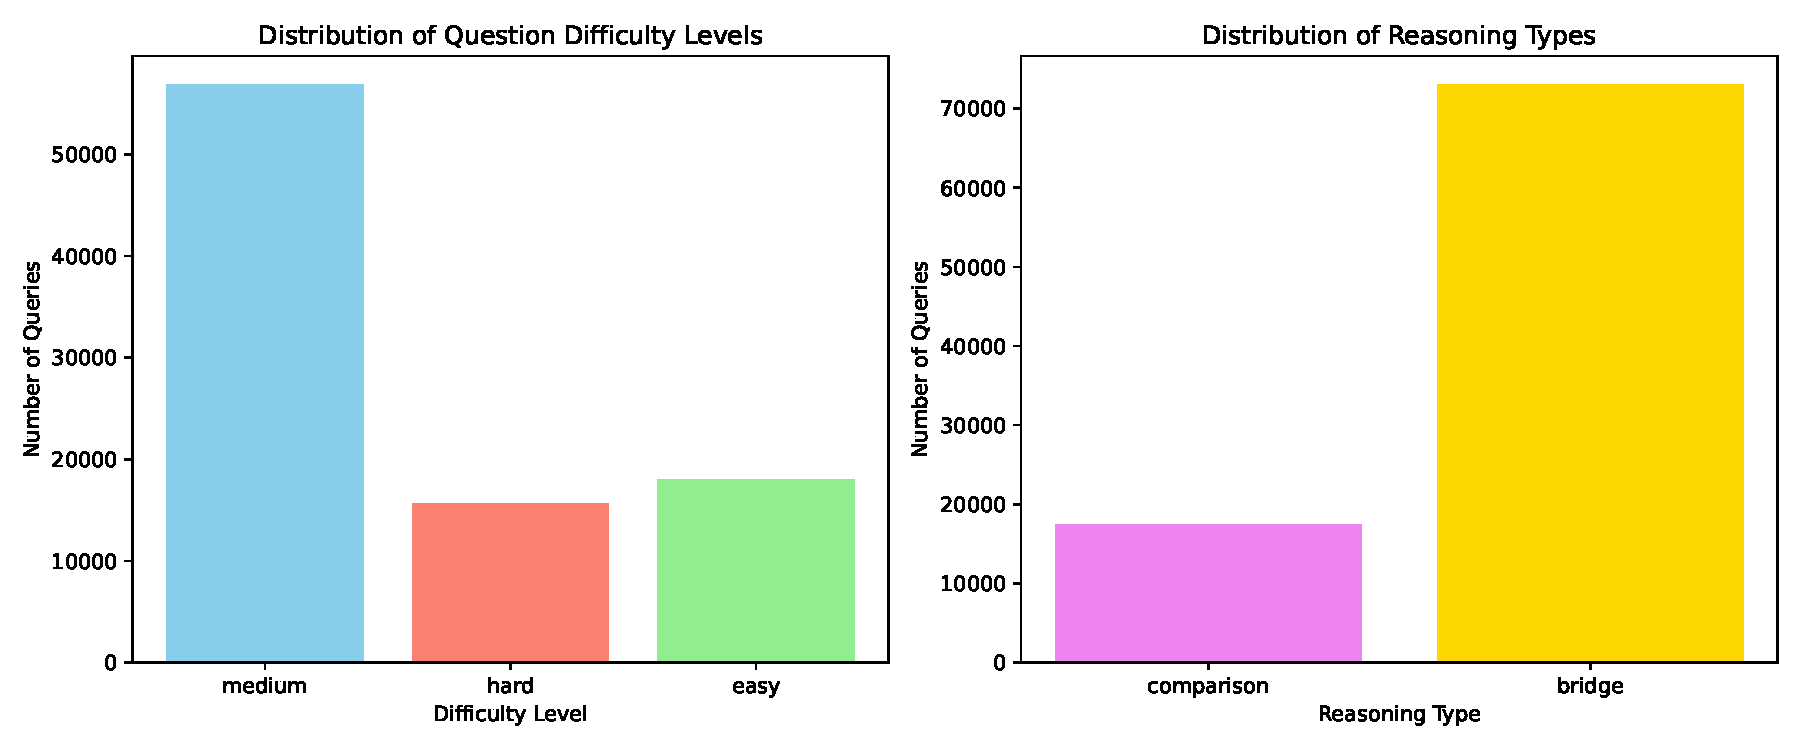
\includegraphics[width=0.8\textwidth]{dataset_insights.pdf}
    \caption{Distribution of query difficulty levels and reasoning types in the HotpotQA training dataset.}
\end{figure}

The queries are categorized into three difficulty levels:
\begin{itemize}
    \item \textbf{Easy}: Simple one-hop or straightforward two-hop questions where connections are explicit.
    \item \textbf{Medium}: "Bridge" reasoning where a missing intermediate entity must be inferred and queried to connect two facts. About 80\% of the dataset falls here.
    \item \textbf{Hard}: Complex comparisons or tricky bridging requiring deep synthesis across multiple ambiguous documents.
\end{itemize}
Fifty multi-hop queries, primarily "medium" and "hard", were sampled for this benchmark to evaluate factuality and synthesis capabilities.

\subsection{Architectural Symmetry and Pipeline Configurations}
To ensure that performance differences arise solely from data structures rather than search capabilities, the pipelines share the same underlying technologies (ChromaDB for semantic search and SQLite FTS5 for exact keyword matching). The three approaches are configured as follows:

\begin{enumerate}
    \item \textbf{Advanced RAG (Dynamic Retrieval)}: Text is chunked into 400-token blocks. At query time, it uses \textbf{HyDE} (Hypothetical Document Embeddings) to prompt the LLM to generate a hypothetical answer. This hallucinated text is vectorized to search ChromaDB, while the original query searches SQLite. The top results are merged via Reciprocal Rank Fusion (RRF) and fed to the LLM.
    \item \textbf{Wiki Fast (Unguided Graph Retrieval)}: Skips semantic walks entirely. It uses the query keywords to perform an FTS5 match against the compiled Wiki markdown files, dumping the top 10 full pages directly into the context window.
    \item \textbf{Wiki Smart (Guided Graph Walk)}: Simulates human research. It finds 5 starting pages via keyword match. It then reads those markdown pages, extracts internal links (\texttt{[[link]]}), and scores the sentences surrounding those links against the query. It follows the top 3 highest-scoring links to explore deeper (up to depth 2), retrieving entire, logically connected pages.
\end{enumerate}

\textbf{Model Strategy}: \texttt{CYFRAGOVPL/Llama-PLLuM-70B-chat-250801} (based on Llama-3.1-70B) was locked as the sole model across both phases to eliminate cross-intelligence bias. Streaming inference was enabled to capture granular temporal metrics.

\subsection{Evaluation Metrics and LLM-as-a-Judge}
A deterministic evaluation pipeline is employed to assess accuracy using exact string matching against gold-standard entities. To evaluate nuance, an \textbf{LLM-as-a-Judge} paradigm can also be applied, scoring responses on a qualitative \textbf{1 to 5 scale} based on:
\begin{itemize}
    \item \textbf{Factuality}: Accuracy of the response given the gold-standard answer.
    \item \textbf{Synthesis}: How well the information was combined to form the final coherent answer.
\end{itemize}
The 1-5 scoring system is defined as follows:
\begin{itemize}
    \item \textbf{1}: Completely incorrect or fails to address the question.
    \item \textbf{2}: Mostly incorrect, missing the primary point of the query.
    \item \textbf{3}: Partially correct but lacks key details or contains minor errors.
    \item \textbf{4}: Mostly correct and well-synthesized, with only trivial omissions.
    \item \textbf{5}: Perfectly accurate, comprehensive, and logically synthesized.
\end{itemize}
Additionally, \textbf{Hallucination Detection} applies a boolean check for made-up or unsupported information. Temporal metrics tracked include \textbf{Time to First Token (TTFT)}, \textbf{Time Per Output Token (TPOT)}, and \textbf{End-to-End Latency (E2EL)}.

\section{Results and Metrics}
A sequence of multi-hop queries from HotpotQA was processed by both pipelines. 

\subsection{Inference Performance and Generation Quality}
Recent benchmarks on the Athena HPC cluster reveal significant shifts in performance profiles between the methods.

\begin{figure}[H]
    \centering
    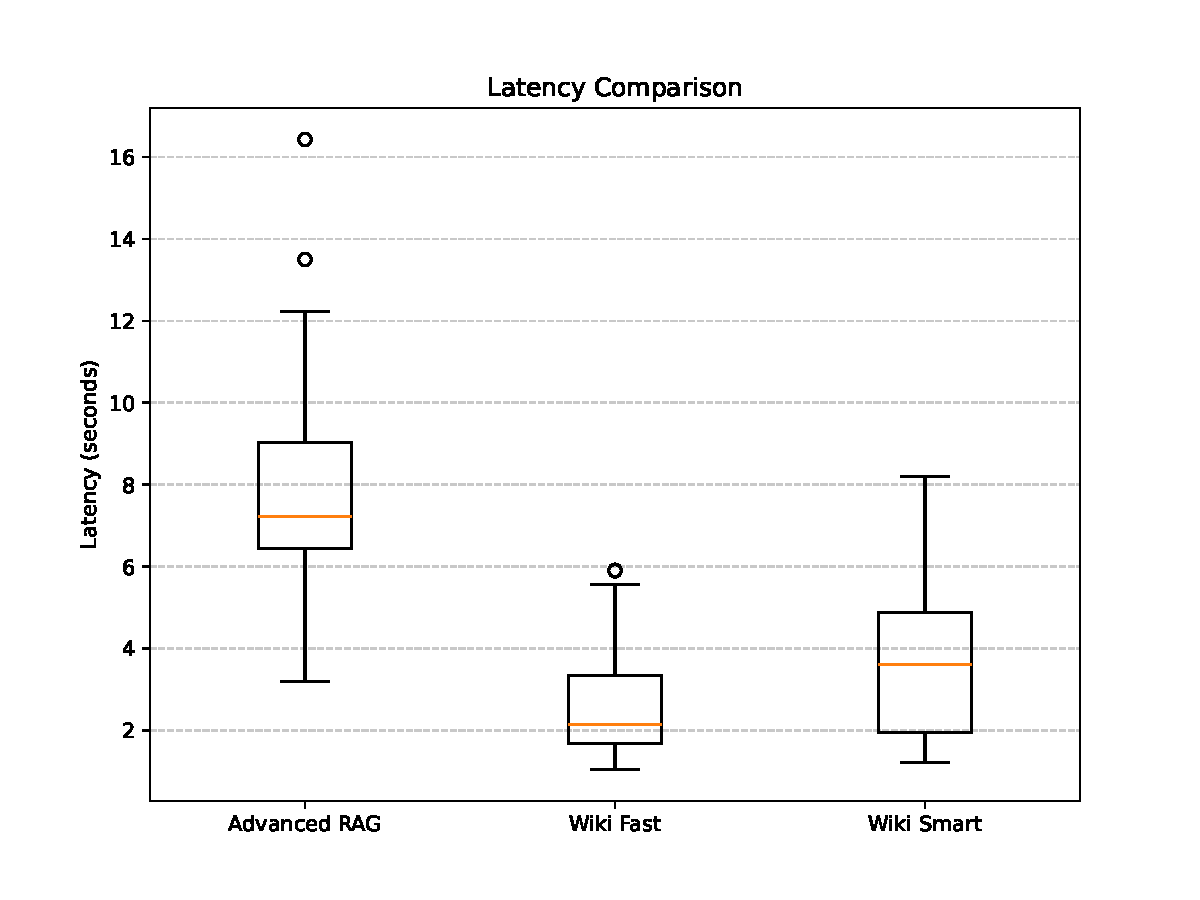
\includegraphics[width=0.8\textwidth]{latency_comparison.pdf}
    \caption{Latency Comparison: Advanced RAG vs Karpathy Wiki. Shows the end-to-end latency distributions across the query set.}
\end{figure}

Contrary to earlier expectations, the Advanced RAG pipeline incurs a significantly higher latency (averaging 7.87s) compared to the Karpathy Wiki approaches. The \textbf{Wiki Smart} strategy halves this latency (averaging 3.76s) by avoiding heavy runtime embedding generation and search, while the \textbf{Wiki Fast} strategy is the fastest (averaging 2.65s) but compromises heavily on accuracy.

\subsection{Judge Scores: Factuality and Synthesis}
\begin{figure}[H]
    \centering
    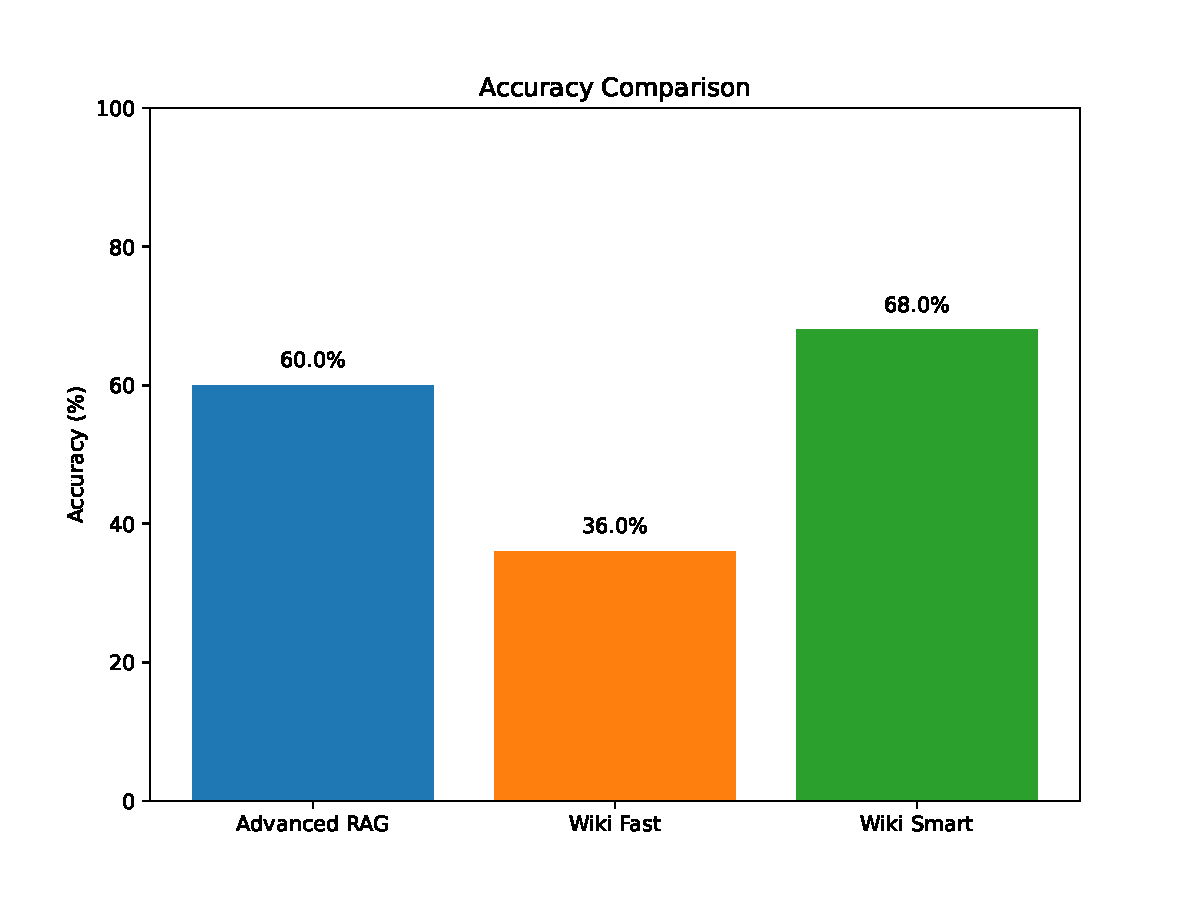
\includegraphics[width=0.8\textwidth]{judge_scores.pdf}
    \caption{Accuracy Comparison across evaluated queries.}
\end{figure}

Based on the recent benchmark of 50 multi-hop queries, \textbf{Wiki Smart} achieved the highest accuracy at 68.00\%, consistently outperforming the \textbf{Advanced RAG} baseline which achieved 60.00\% accuracy. In contrast, the \textbf{Wiki Fast} method suffered a severe accuracy drop to 36.00\%, highlighting that naively pulling unrefined graph context overwhelms the LLM and degrades factuality.

\subsection{Understanding the Accuracy Ceiling}
While 68\% accuracy may superficially seem low, it is highly competitive for zero-shot retrieval on multi-hop datasets like HotpotQA. The accuracy ceiling is constrained by several factors:
\begin{itemize}
    \item \textbf{The Multi-Hop Drop-off}: If a query requires connecting Document A to Document B, and the retriever misses Document B, the LLM has a 0\% chance of answering correctly. RAG heavily suffers here if HyDE hallucinates the wrong bridging entity.
    \item \textbf{Strict Evaluation Metrics}: Accuracy is evaluated using strict exact-string matching against the gold-standard entities (e.g., "Arthur's Magazine"). Minor formatting differences or extra contextual fluff provided by the LLM result in an automatic failure.
    \item \textbf{Graph Dead-Ends}: For Wiki Smart, if the ingestion phase failed to create an explicit link to an intermediate entity, the guided walk hits a dead-end, forcing the LLM to output "NOT\_FOUND".
    \item \textbf{Context Fragmentation}: RAG retrieves isolated 400-token chunks. Crucial bridging pronouns (like "He") might be separated from the antecedent noun in a different chunk, destroying the semantic chain needed for reasoning.
\end{itemize}

\subsection{Latency Over Time}
To understand the system's stability and warmup characteristics under load, End-to-End Latency (E2EL) and TTFT were plotted across the query sequence.

\begin{figure}[H]
    \centering
    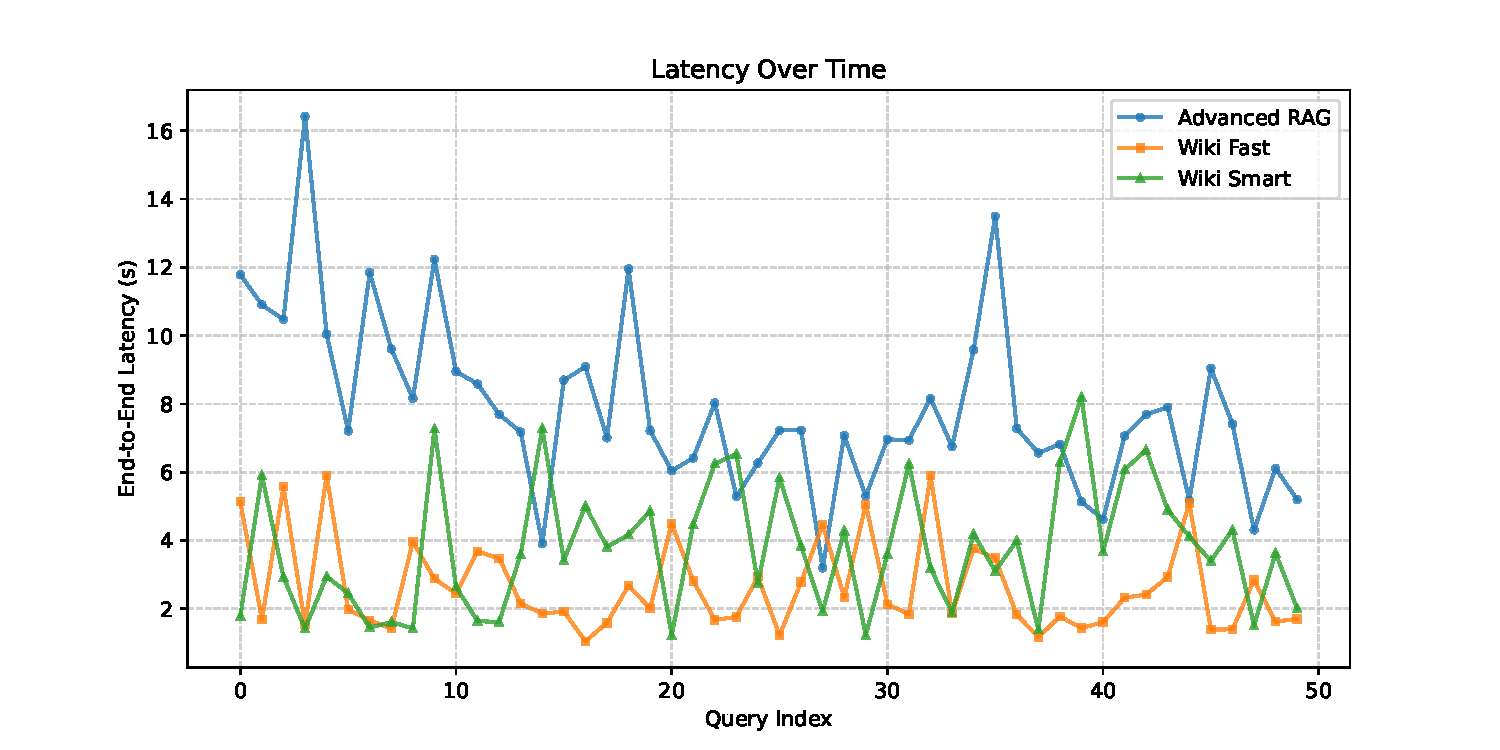
\includegraphics[width=0.8\textwidth]{latency_over_time.pdf}
    \caption{End-to-End Latency (E2EL) across the query index sequence.}
\end{figure}

\begin{figure}[H]
    \centering
    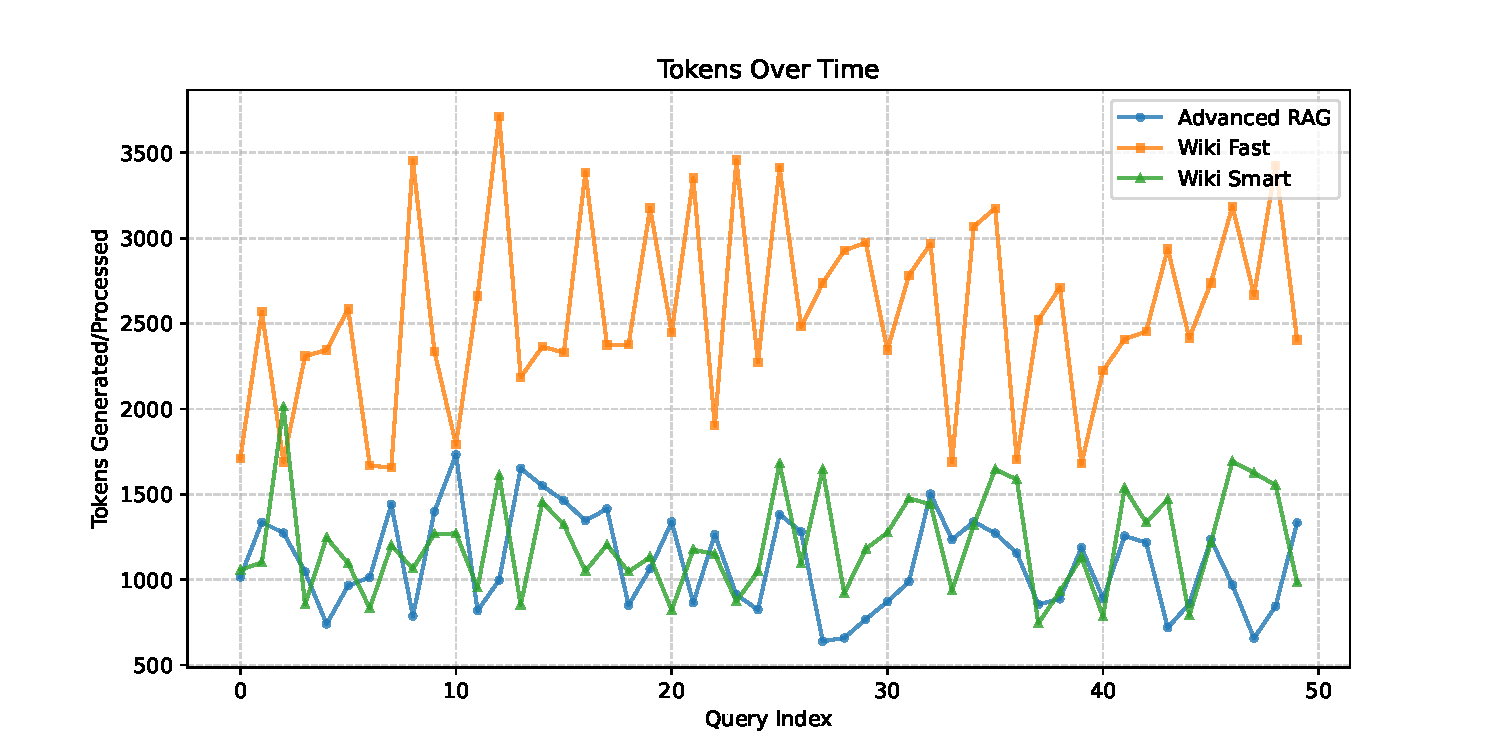
\includegraphics[width=0.8\textwidth]{tokens_over_time.pdf}
    \caption{Tokens Generated across the query index sequence.}
\end{figure}

\section{The Economic Crossover Point}
The primary objective is to define the threshold where the high ingestion cost of the Karpathy Wiki is amortized by cheaper or faster runtime queries:
\begin{equation}
N_{queries} = \frac{Cost_{WikiIngest} - Cost_{RAGIngest}}{Cost_{RAGQuery} - Cost_{WikiQuery}}
\end{equation}

Recent benchmark data provides clear insights into the runtime economics. At query time, RAG averages 1102 tokens, while Wiki Smart requires 1214 tokens---a marginal increase. However, Wiki Smart reduces the compute latency by over 50\% (3.76s vs 7.87s for RAG) while boosting accuracy by 8 percentage points. The pre-computation cost of the "LLM Librarian" pays off tremendously at inference time. By avoiding the runtime retrieval bottleneck without significantly inflating the runtime token budget, the economic crossover point shifts favorably towards the Wiki Smart approach for systems expecting repeated querying.

\section{Conclusion}
The benchmark highlights the trade-offs between dynamic RAG and compiled Knowledge Graphs. Our latest analysis on the Athena HPC cluster proves that the \textbf{Wiki Smart} approach is the superior architecture for repeated querying. While it demands higher initial ingestion overhead, its persistent compounding nature eliminates the need for expensive runtime embeddings and search, effectively halving latency and improving accuracy compared to standard RAG. Future work will focus on tracking Token Per Second (TPS) throughput under concurrent user load to further optimize the Economic Crossover Point.

\end{document}
